\chapter{Experimental results}\label{ch:Ch.5}
This chapter discusses the results achieved by the model described previously in \textit{Chapter \ref{ch:Ch.4}} through the tests performed.
Then a comparison between the proposed model, other techniques used in testing and the $BRI_2$ is shown.
The results include a subset of airports where the accuracy of the model was verified.

\section{Model results}\label{results}
The proposed model has been tested on a subset of airports contained in the available dataset including Florence, Pisa, Bologna, Milan-Malpensa, Milan-Linate, Catania, Brescia, Verona.
An observation window of 15 days was used for the test to provide the model with enough time information. These are very important due to the seasonal trend of birdstrike events. Observations of 15 days showed promising performance on the tests.
The tests were performed inclusively between the year 2012 and 2018. The resulting dataset was split 75\%:
\begin{itemize}
    \item The train-set is composed of 1852 days.
    \item The test-set is formed by 575 days.
\end{itemize}
The model has been trained for 600 epochs. Additional epochs may cause the model to overfit.
The learning rate chosen was $1\times10^{-5}$ and to guarantee the stability of the correlation the learning rate scheduler multiplies it by 0.75 every 200 epochs, as discussed in \ref{Loss_function}.
The Custom loss was set with $\sigma = 0.1$.
The Spearman correlation was chosen to evaluate the model's performance, and quantitative results (correlation) and qualitative results, i.e. the comparison between Ground Truth and the new risk-index, will be shown below.


\begin{figure}
	\centering
	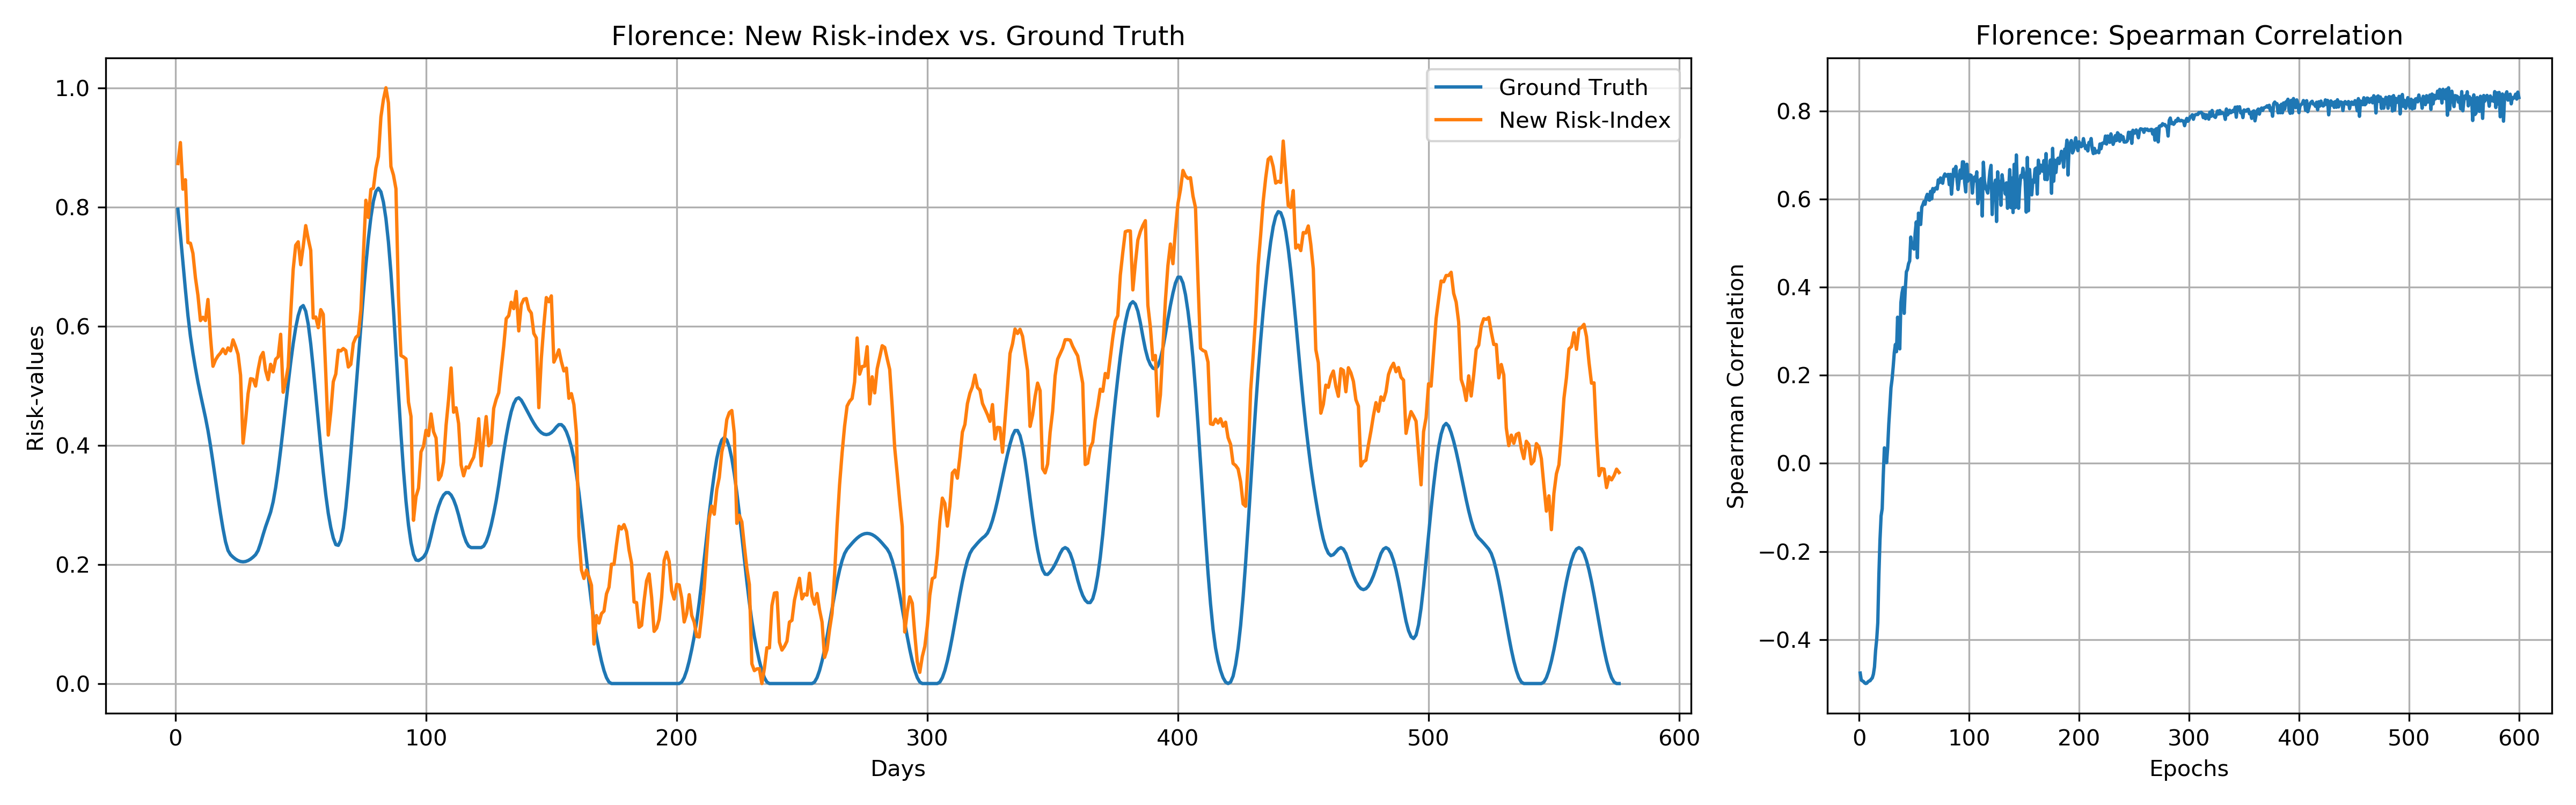
\includegraphics[width=14cm]{img/FI.png}	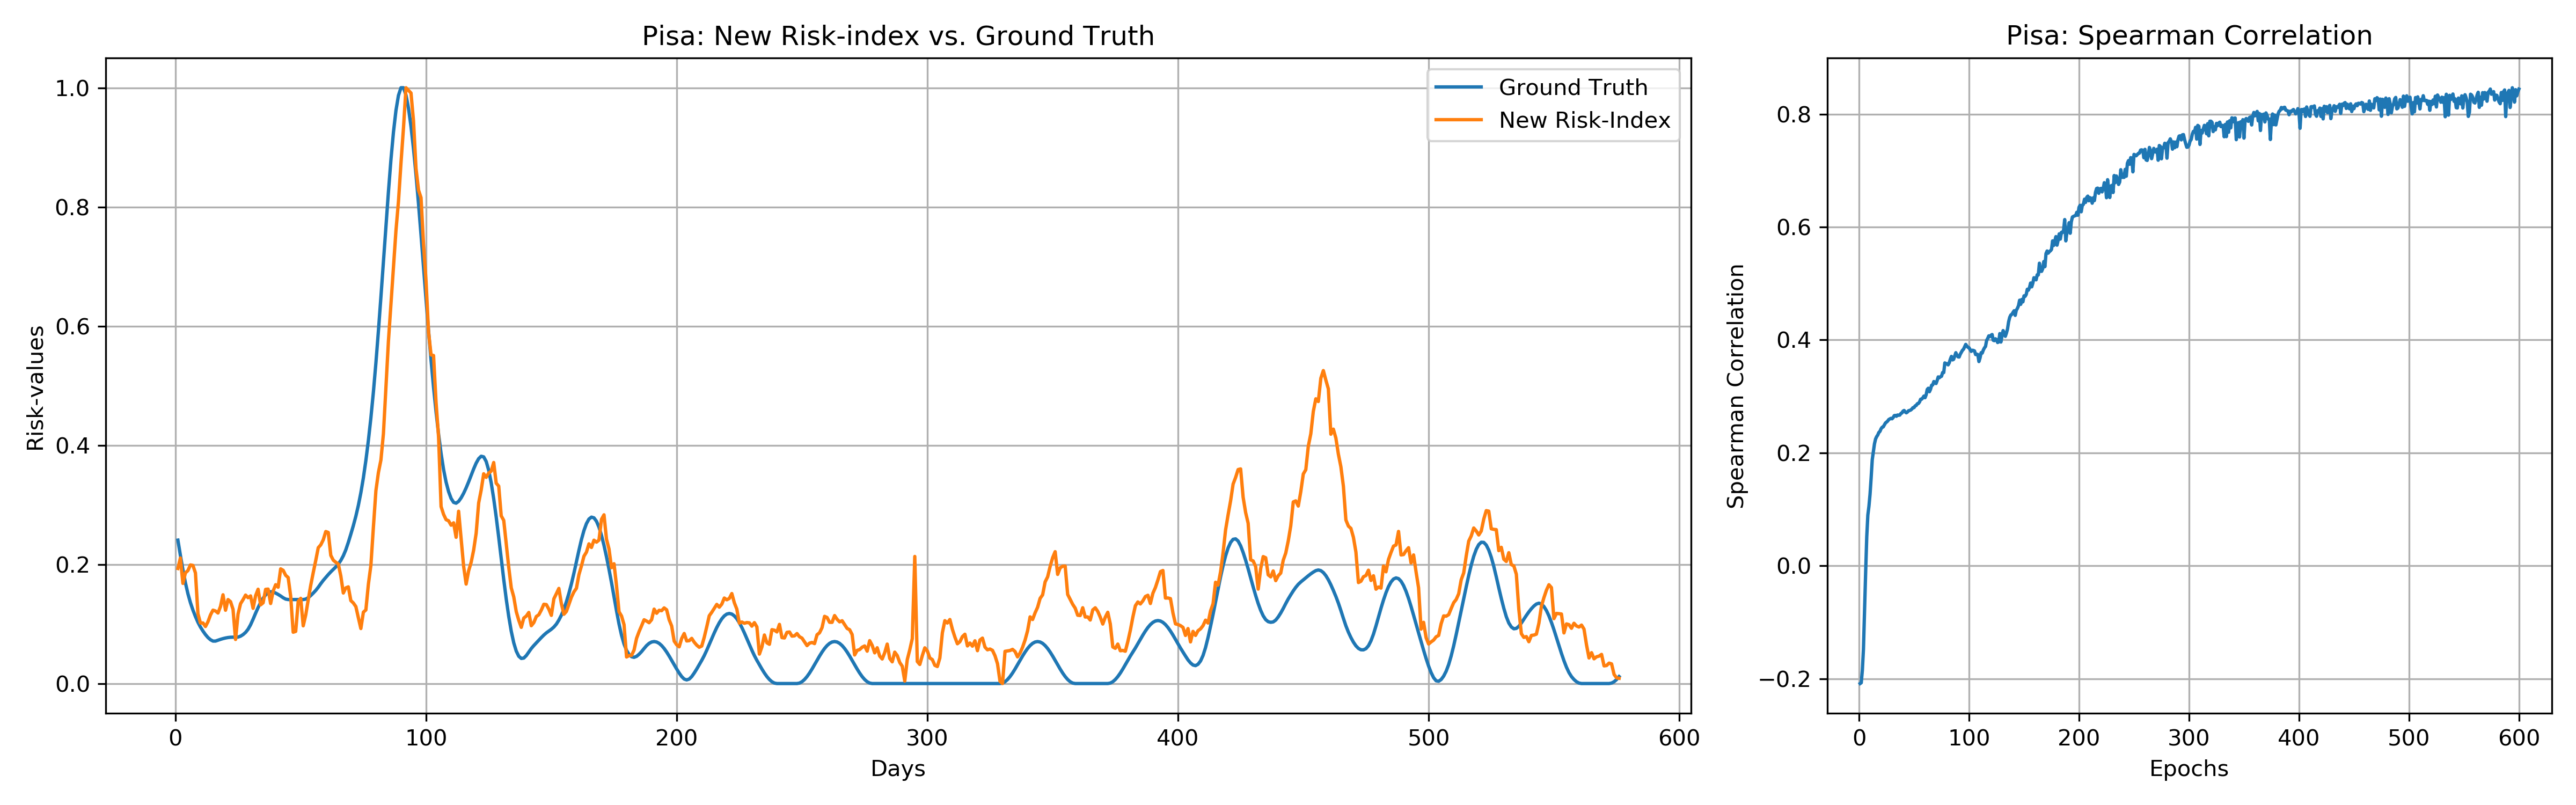
\includegraphics[width=14cm]{img/PSA.png}
	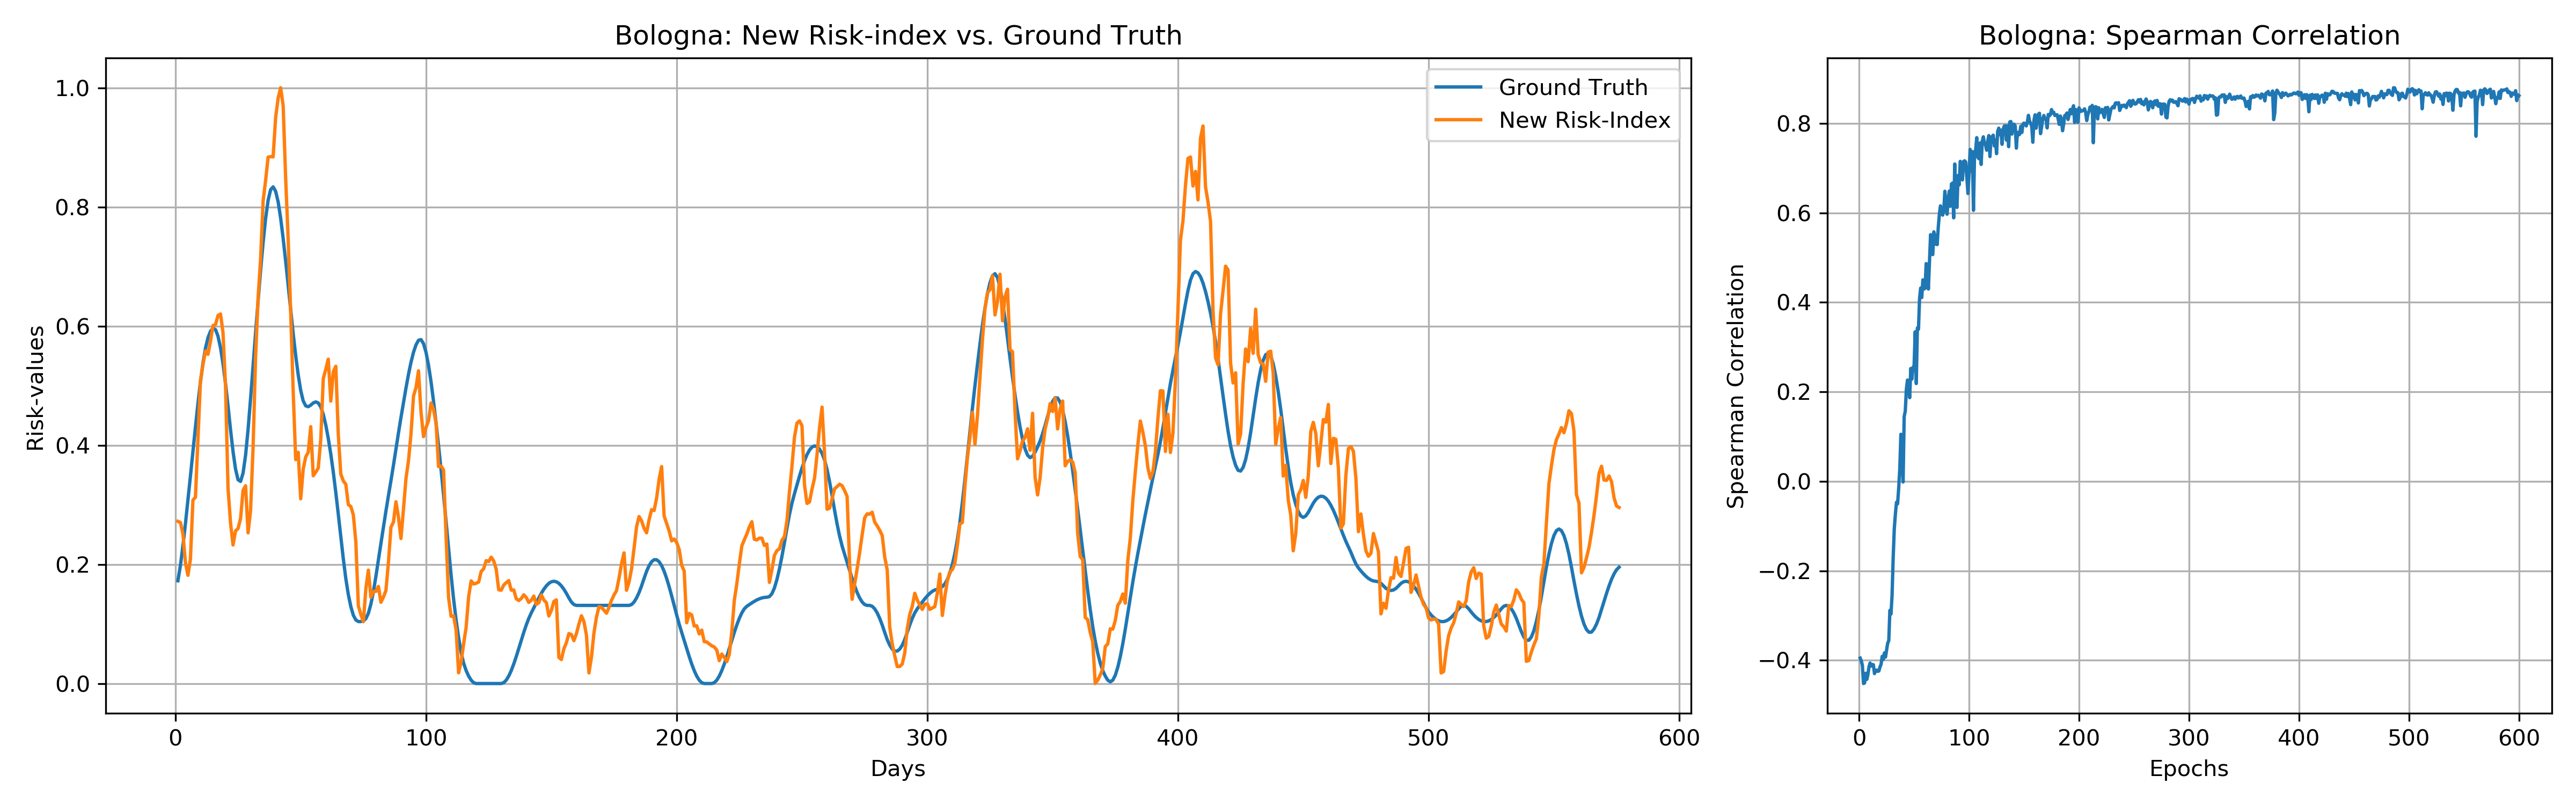
\includegraphics[width=14cm]{img/BO.png}
	\caption{Results for the airports of Florence, Pisa and Bologna. On left the comparison between Ground Truth and the new risk-index, and on right the Spearman correlation. The proposed model is a very accurate risk predictor, the correlation with birdstrike events is high with values of 0.83, 0.84, 0.86.}
	\label{FI_PSA_BO_results}
\end{figure}

\begin{figure}
	\centering
	\includegraphics[width=14cm]{img/malpensa.png}
	\includegraphics[width=14cm]{img/catania.png}
	\includegraphics[width=14cm]{img/verona.png}
	\caption{Results for the airports of Milan-Malpensa, Catania and Verona. On left the comparison between Ground Truth and the new risk-index, and on right the Spearman correlation. The proposed model is a very accurate risk predictor, the correlation with birdstrike events is high with values of 0.82, 0.86, 0.87.}
	\label{MAL_CA_VE_results}
\end{figure}

\begin{figure}
	\centering
	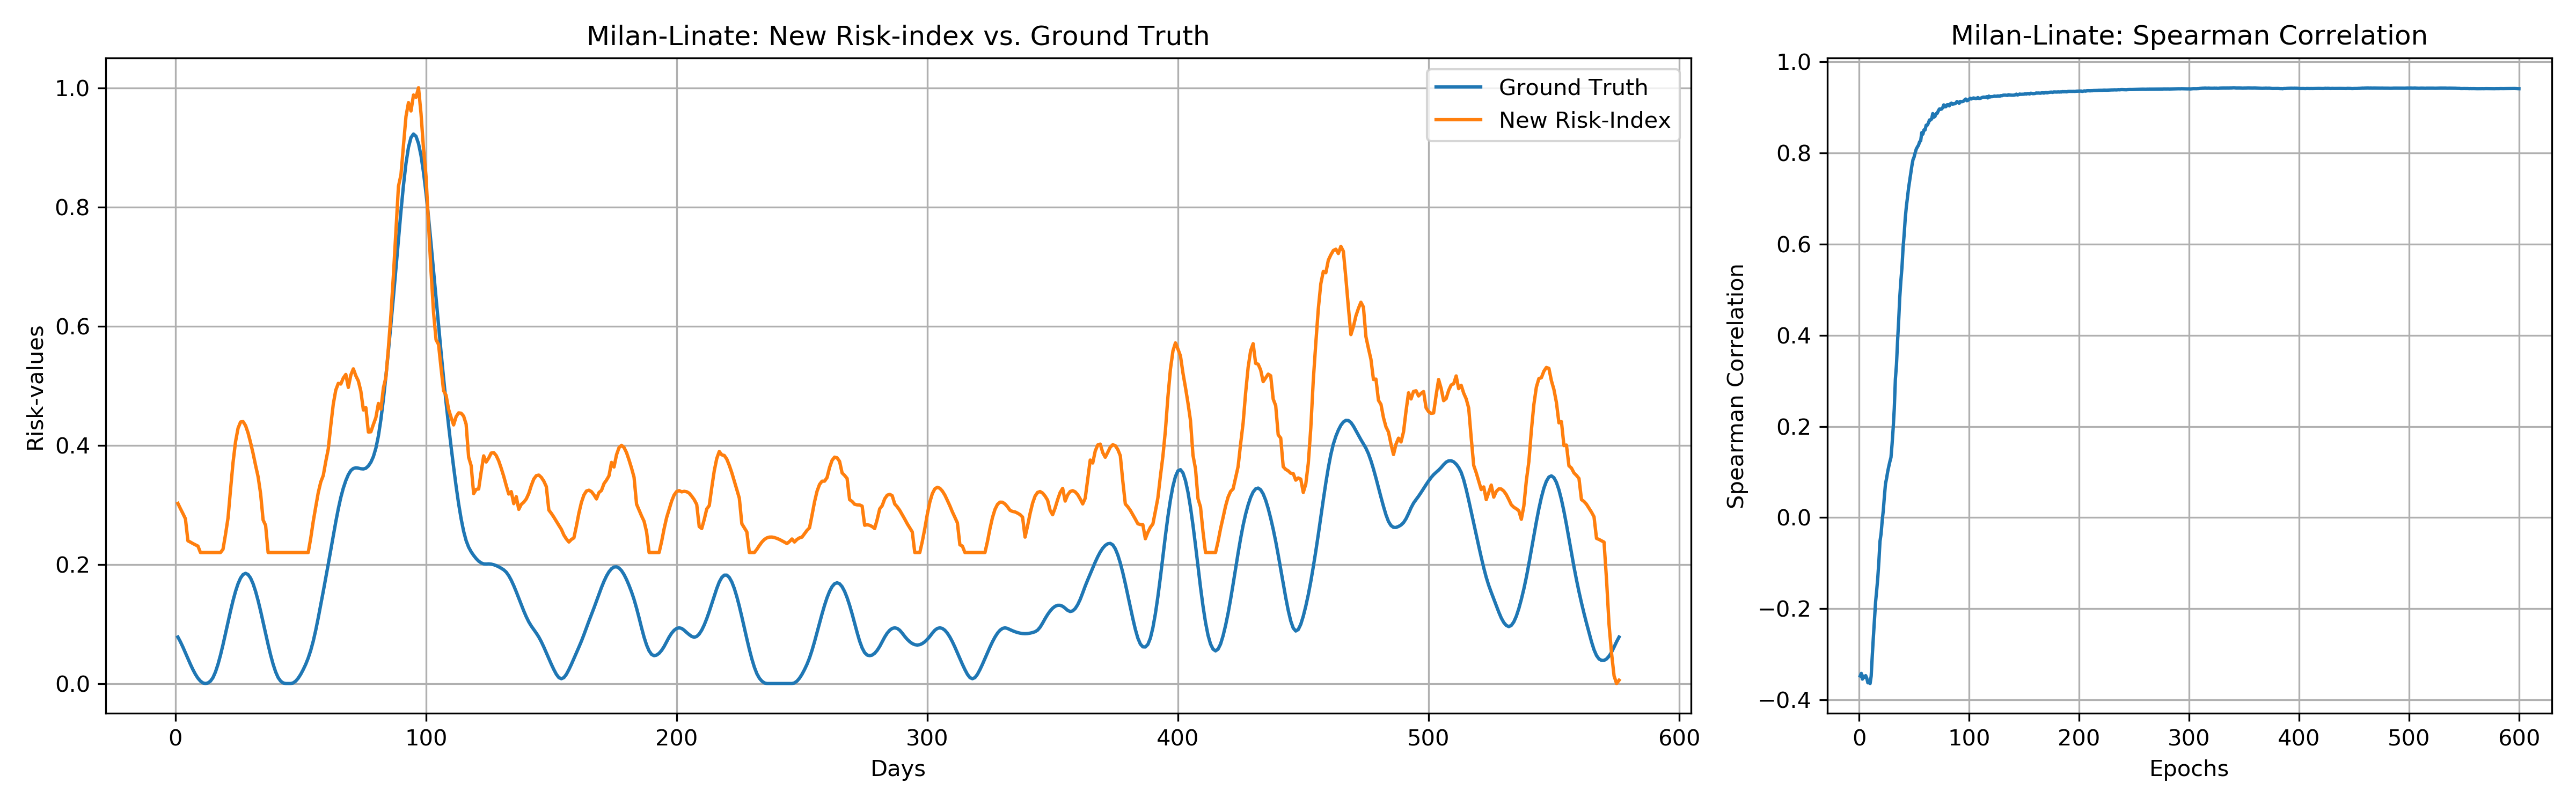
\includegraphics[width=13.8cm]{img/LI.png}
	\caption{Milan-Linate airport results. On left the comparison between Ground Truth and the New Risk-Index, and on right the Spearman correlation.  The proposed model is a very accurate risk predictor, the correlation with birdstrike events is high with a value of 0.94.}
	\label{LI_results}
\end{figure}


The figures \ref{FI_PSA_BO_results}, \ref{MAL_CA_VE_results} and \ref{LI_results} show how the proposed model is able to predict the periods of birdstrike events with very good approximation. The model is able to interpret which are the most dangerous periods and provide a risk value consistent with the events historically occurred.
This is confirmed by the Spearman correlation values for the airports tested.
These values are very promising and indicate an effective correlation between birdstrike events and the new risk-index generated by the model.
Only Brescia Airport did not return good results, with a low correlation.  The data regarding birdstrikes at this airport are insufficient and poorly reported for the training of the model.
In particular, the figures \ref{FI_PSA_BO_results}, \ref{MAL_CA_VE_results} and \ref{LI_results} show on the left the comparison between the Ground Truth and the new risk index, and on the right the Spearman correlation value for each test epoch.
In Table \ref{tab-model_acc} it is possible to observe the results quantitatively for each analyzed airport:

\begin{table}
	\centering
	\scalebox{1.0}{
	\begin{tabular}{@{}ccc@{}}
		\toprule
		Airport & Proposed Model & $BRI_2$ \\ 	\midrule
		Florence & 0.83 & 0.17\\
		Pisa & 0.84 & 0.74\\
		Bologna & 0.86 & 0.26\\
		Milan-Malpensa &  0.82 & -0.14\\
		Milan-Linate &  0.94 & -0.28\\
		Verona & 0.87 & 0.6\\
	    Catania & 0.86 & 0.49\\
	    Brescia & -0.2 & 0.31\\    \bottomrule
	\end{tabular}}
	\caption{Proposed Model accuracy (Spearman correlation) against the results obtained with $BRI_2$.}
	\label{tab-model_acc}
\end{table}

\section{Results comparison}
The results of the proposed model have been presented in the previous section.
Other models were previously tested as possible candidates to solve the task. These models differ in architecture or are variants of the model already described.
The results of the model must also be compared with $BRI_2$. This comparison is of relevant importance because the goal of the model is to improve the Spearman correlation between $BRI_2$ and birdstrike events. 
The other models evaluated and tested are:

\begin{itemize}
    \item $BRI_2$: the current risk index adopted in Italian airports
    \item LSTM: first appreciable results obtained with Machine Learning techniques on which the following choices were based.
    \item Siamese-LSTM with Custom loss, presented in \ref{Loss_function}, learning rate = $1\times10^{-4}$: first attempt to introduce margin ranking loss to increase the accuracy achieved by the previous model.
    \item Siamese-LSTM with Custom loss, learning rate = $1\times10^{-5}$: model tested to stabilize the Spearman correlation.
\end{itemize}

The Figure \ref{comparison1} shows the comparison of the results of the tested models.
The comparison has been made for the subset of airports that have been analysed. For each airport the Spearman correlation value found with the tests executed for the evaluated models specified above are shown.
It is important to remember that the correlation values of LSTM, Siamese-LSTM(learning rate = $1\times10^{-4}$) and Siamese-LSTM(learning rate = $1\times10^{-5}$) are unstable as discussed in \ref{MRL}.
The comparison shows that the proposed model achieves a higher correlation than the other models tested.
In particular, the most significant comparison is with the $BRI_2$. The proposed model has a better performance than the $BRI_2$ with the exception of Brescia but as discussed in \ref{results} the available birdstrike data are not sufficient to train the model.

The results shown in this chapter are encouraging. The next chapter \textit{Chapter \ref{ch:Ch.6}} will discuss the goals achieved given these results, their importance and the improvements achieved.

\begin{figure}
	\centering
	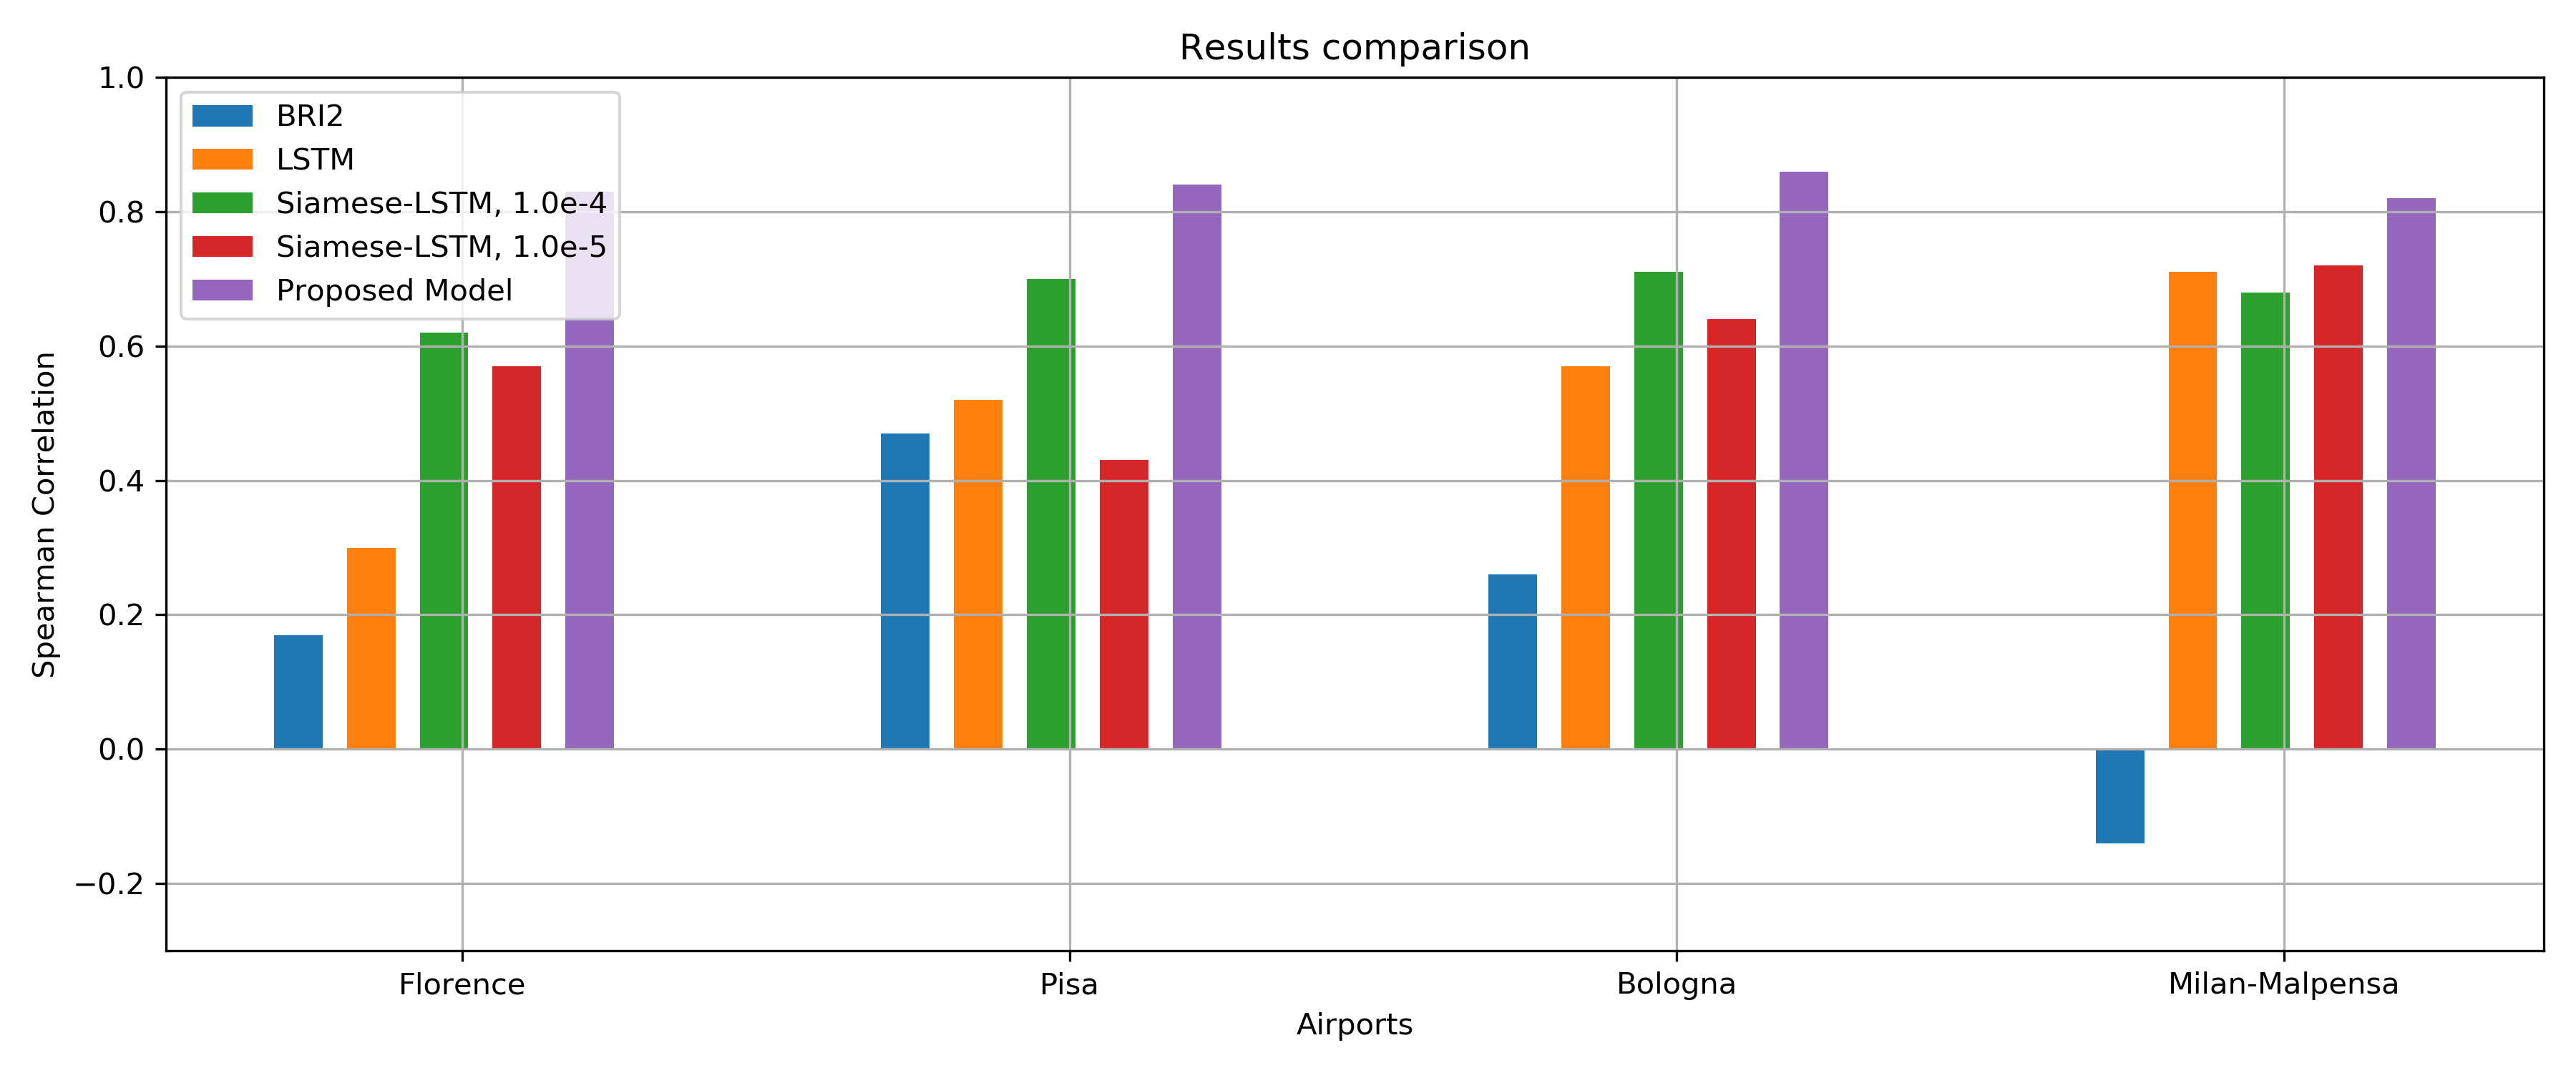
\includegraphics[width=13.8cm]{img/comparison1.png}
	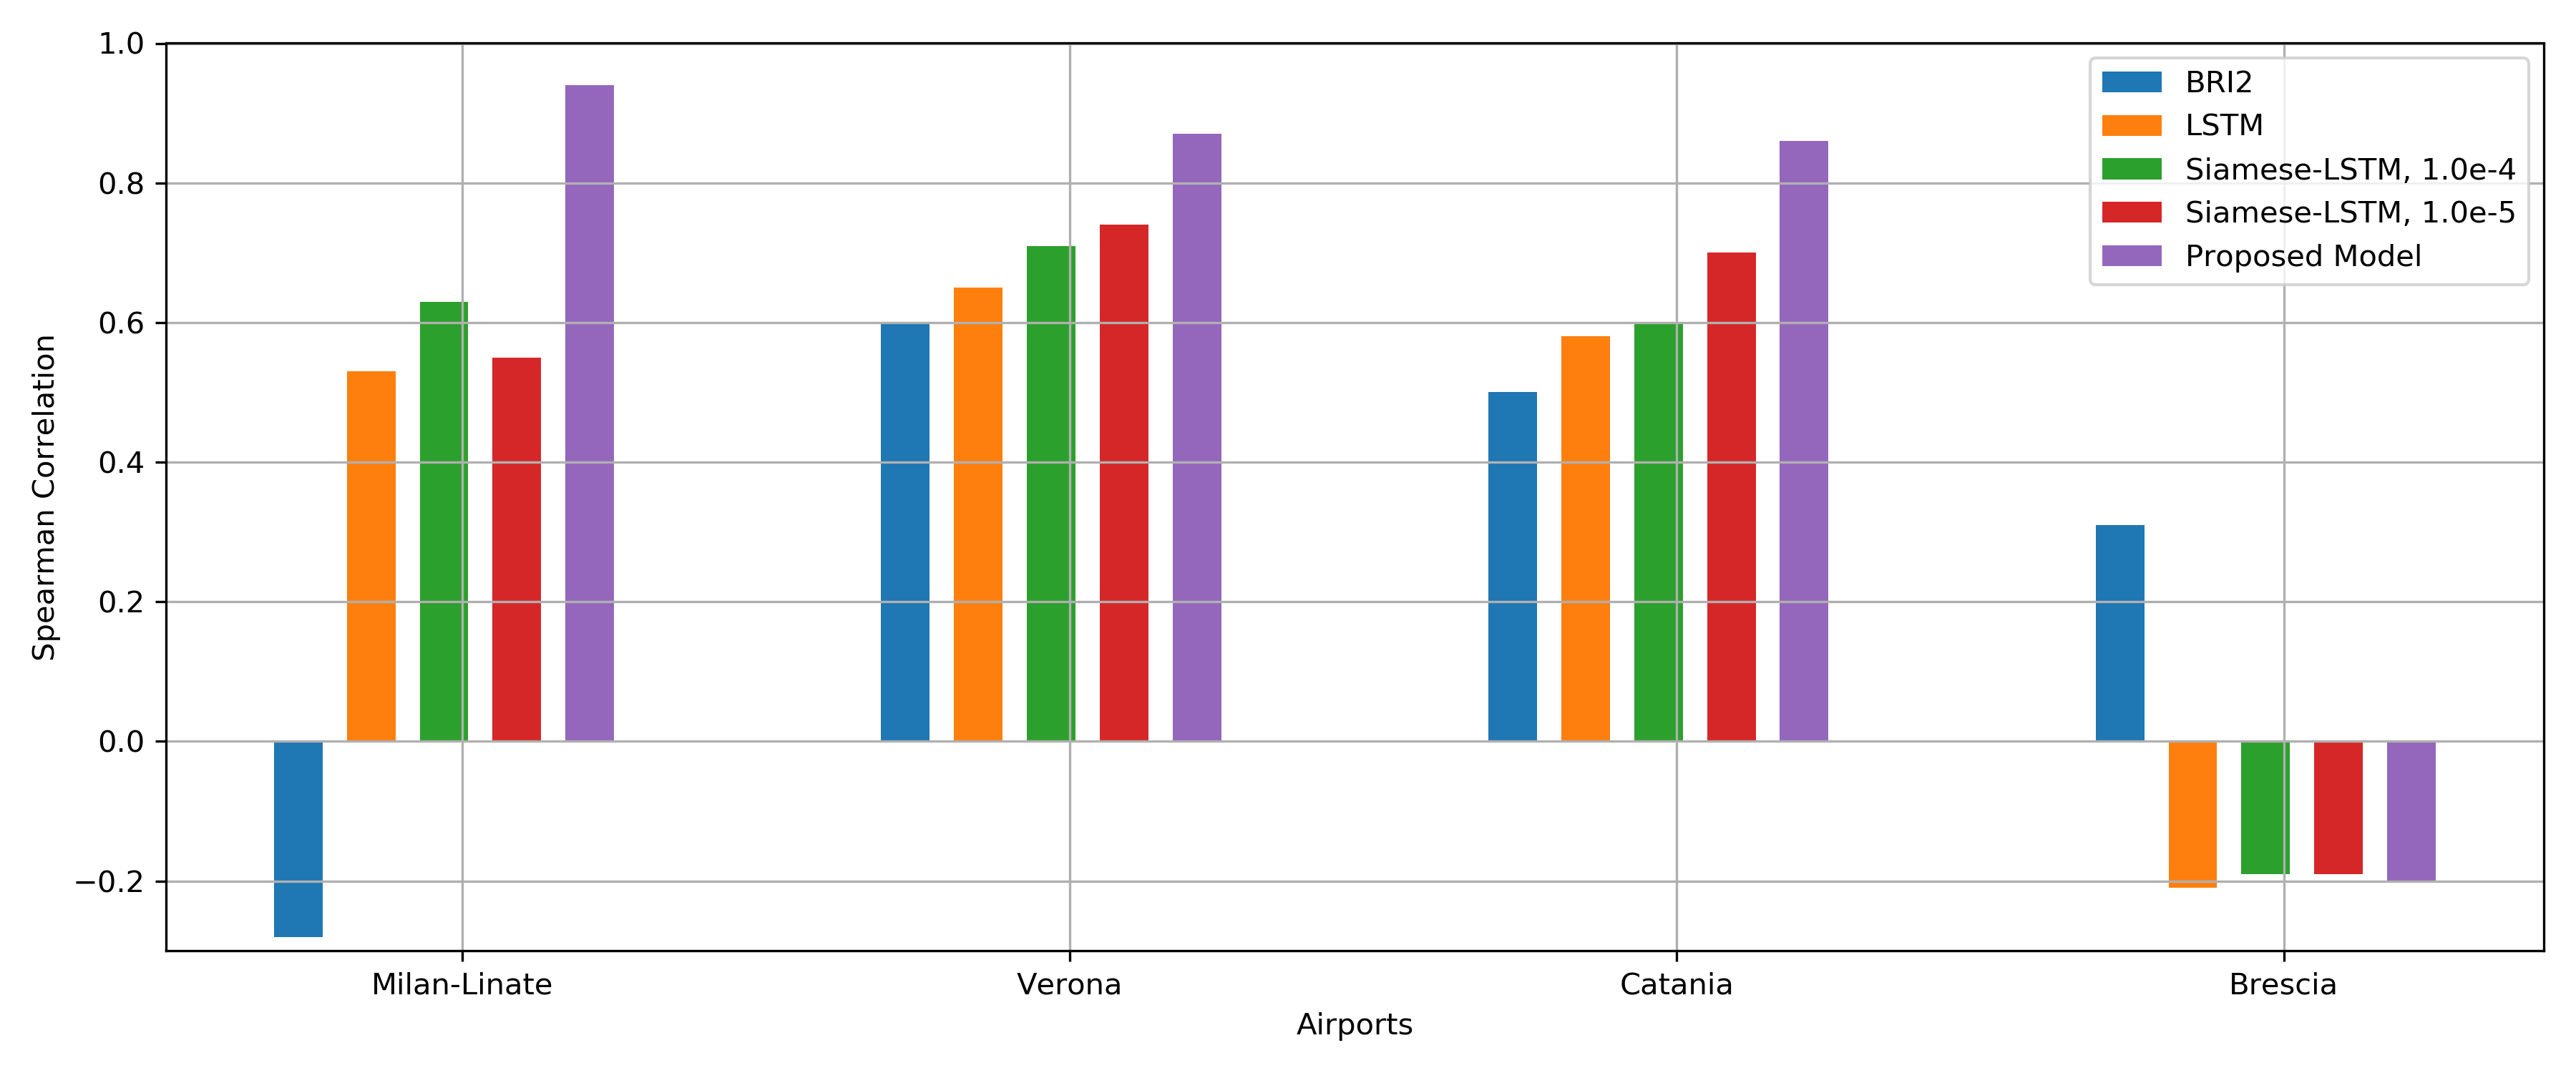
\includegraphics[width=13.8cm]{img/comparison2.png}
	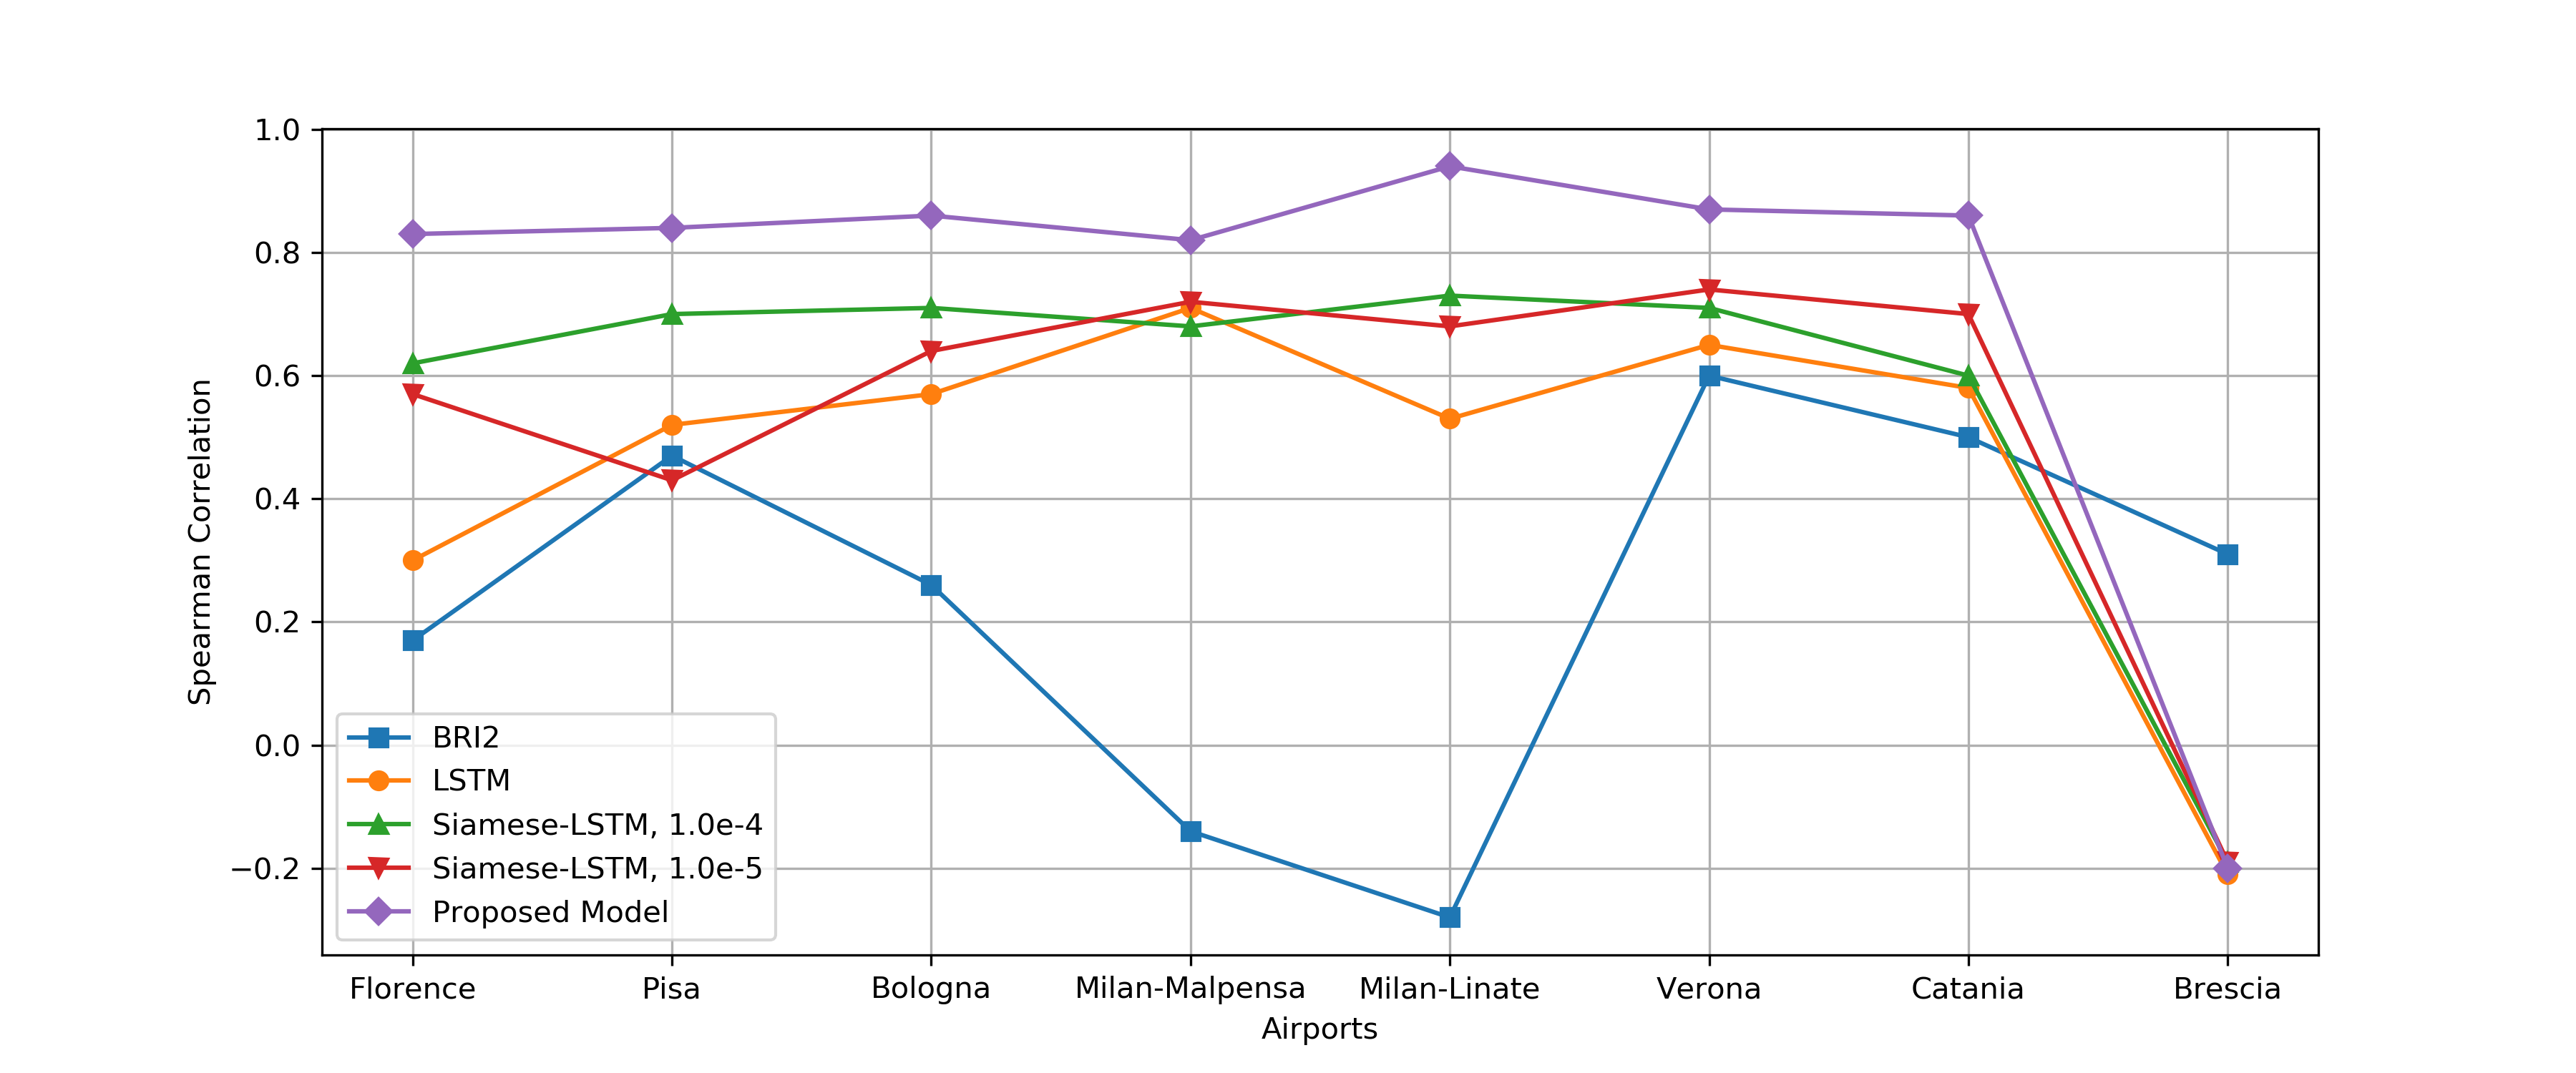
\includegraphics[width=14cm]{img/comparison3_2.png}
	\caption{Models results comparison for Florence, Pisa, Bologna, Milan-Malpensa, Milan-Linate, Verona, Catania and Brescia airports. The figure illustrates how the proposed model shows better performance than the $BRI_2$ and is the data-driven model most related to the birdstrike events collected.}
	\label{comparison1}
\end{figure}
